
\begin{frame}{Le changement climatique}{Le réchauffement et ses conséquences}

\begin{figure}
	\centering
	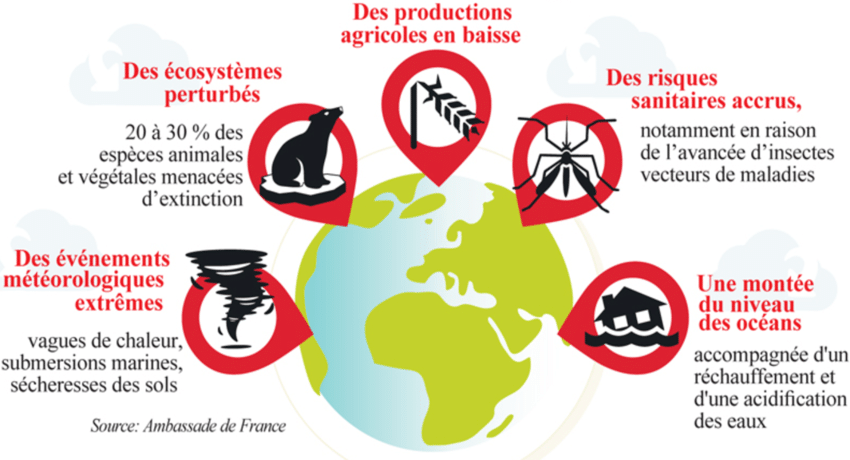
\includegraphics[scale=0.37]{Feathergraphics/effetChgmtClimat.png}
\end{figure}

\end{frame}
\begin{frame}{Pollution liée à l'activité humaine}{et focus sur le numérique}
\begin{figure}[h!]
\begin{minipage}[b]{0.5\linewidth}
\begin{block}{$CO_2$ d'origine humaine}
	\begin{itemize}
		\item Production energétique : $39\%$
		\item Transport : $23\%$			
		\item Industrie : $22\%$		
		\item Résidentiel : $10\%$		
		\item Tertiaire : $4\%$	
		\item Agriculture : $2\%$
	\end{itemize}
\end{block}
	
\end{minipage}\hfill
\begin{minipage}[b]{0.45\linewidth}   
\begin{tikzpicture}
\node[blue] at (1,3)   (a) {Fabrication};
\node[blue] at (3.5, 1.5)   (b) {Utilisation};
\node[blue] at (1, 0)   (c) {Destruction};

\draw[->,>=latex, line width=1mm,color=blue!50] (a) to[bend left=50] (b);
\draw[->,>=latex, line width=1mm,color=blue!50] (b) to[bend left=50] (c.east);
\draw[->,>=latex, line width=1mm,color=blue!50] (c.west) to[bend left=50] (a.west);
\node (ordi) at (1.4,1.5) {
\includegraphics[scale=0.08]{Feathergraphics/ordi.png}};
\end{tikzpicture}


\end{minipage}

\begin{alertblock}{Question}
	Quelle est la part du numérique ?~\cite{ImpactNumerique}~\cite{greenpeace}
\end{alertblock}
\end{figure}

\end{frame}

\begin{frame}{Pollution liée à l'activité humaine}{et focus sur le numérique}
	\begin{figure}[h!]
		\begin{minipage}[b]{0.5\linewidth}
			\begin{block}{Origine humaine}
				\begin{itemize}
					\item \textcolor{blue}{Production energétique : $39\%$}%20pourcent 
					\item Transport : $23\%$			
					\item Industrie : $22\%$		
					\item Résidentiel : $10\%$		
					\item Tertiaire : $4\%$	
					\item Agriculture : $2\%$
				\end{itemize}
			\end{block}
			
		\end{minipage}\hfill
		\begin{minipage}[b]{0.45\linewidth}   
			\begin{tikzpicture}
			\node[blue] at (1,3)   (a) {Fabrication};
			\node[blue] at (3.5, 1.5)   (b) {Utilisation};
			\node[blue] at (1, 0)   (c) {Destruction};
			
			\draw[->,>=latex, line width=1mm,color=blue!50] (a) to[bend left=50] (b);
			\draw[->,>=latex, line width=1mm,color=blue!50] (b) to[bend left=50] (c.east);
			\draw[->,>=latex, line width=1mm,color=blue!50] (c.west) to[bend left=50] (a.west);
			\node[opacity=0.3] (ordi) at (1.4,1.5) {
\includegraphics[scale=0.08]{Feathergraphics/ordi.png}};
			\node (ordi2) at (1.4,1.5) {\Huge \textbf{$4\% \nearrow$} };
			\end{tikzpicture}
			
			
		\end{minipage}
	
	\begin{block}{Pourquoi ?}
	\cite{bachelet2007global}~\cite{webeco}~\cite{shift}	%34 000 000 000 de smartphones, consoles et télés.
	\end{block}
	\end{figure}
	
\end{frame}

